\documentclass[../../deep_learning_notes.tex]{subfiles}
\begin{document}
%%%%%%%%%%%%%%%%%%%%%%%%%%%%%%
\section{Optimizers}
Optimizers implement different techniques for performing gradient descent and aim to solve problems of noisy updates to perform smooth descent and faster convergence.


%%%%%%%%%%%%%%%%%%%%%%%%%%%%%%
\subsection{Stochastic Gradient Descent (SGD)}
The most basic version of gradient descent, here we take one example from the data set, calculate the loss, and perform one iteration of backprop.
\begin{lstlisting}
while($\lVert w_{t} - w_{t-1} \rVert > \epsilon$){
    for($i = 1, \ldots, N$){
        $w_{t} = w_{t-1} - \eta \nabla_{w} L(w_{t-1}, X_{i}, y_{i})$
    }
}
\end{lstlisting}
where $\eta$ is the learning rate. Because it uses just one example for backprop, the updates can be very noisy, and getting the value of $\eta$ correct can be difficult. $\epsilon$ is a pre defined threhold such that we will stop performing updates once the difference in weights is below this value.\newline
As an implementation note, the data indices are usually shuffled in a random order to avoid introducing any kind of bias to the system. (For instance, the data could be arranged such that all instances of one class come before another. In this case, the model will see a single class for a long time and will not learn to distinguish between the two, since it only needs to output one class for a long time.\newline

Stochastic gradient descent is commonly used when we are doing online learning. At a time, we can only get a single example and update the network weights using only this example.

\begin{figure}[h]
    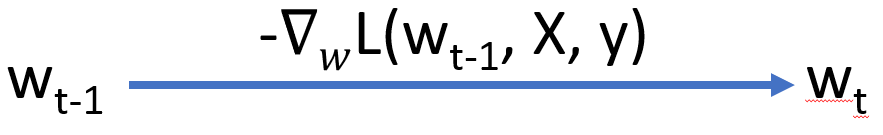
\includegraphics[scale=0.4]{momentum_1}
    \centering
    \caption {Vector representation of SGD}
    \label{fig:momentum_1} %\ref{fig:momentum_1}
\end{figure}

%%%%%%%%%%%%%%%%%%%%%%%%%%%%%%
\subsection{Batch Gradient Descent}
An improved version of stochastic gradient descent, here we use the entire data available to perform gradient descent.
\begin{lstlisting}
while($\lVert w_{t} - w_{t-1} \rVert > \epsilon$){
    $w_{t} = w_{t-1} - \eta \frac{1}{N} \sum_{i=1}^{N}\nabla_{w} L(w_{t-1}, X_{i}, y_{i})$
}
\end{lstlisting}
where $N$ is the size of data set. Since we are using the entire data, the value of mean gradient will be accurate and we can use a high learning rate. In general, \textbf{higher the number of data points used for gradient descent, the more confident we are in the value of gradient, and higher the learning rate can be}. This method requires a lot of calculations to perform updates and thus may not be feasible in case of large data sets.


%%%%%%%%%%%%%%%%%%%%%%%%%%%%%%
\subsection{Mini-Batch Gradient Descent}
This is similar to batch gradient descent, but does the updates using only a subset of the data which is also called a batch. We divide the entire data into such equal sized chunks and one complete iteration will involve performing updates on all such batches
\begin{lstlisting}
while($\lVert w_{t} - w_{t-1} \rVert > \epsilon$){
    for(batch $B$ in data){
        $w_{t} = w_{t-1} - \eta \frac{1}{b} \sum_{i=1}^{b}\nabla_{w} L(w_{t-1}, X_{B,i}, y_{B,i})$
    }
}
\end{lstlisting}
where $b$ is the batch size and the mean is calculated over the entire batch $B$. Learning rate will change based on the size of batch. Due to the small batch size, we can now work with much larger data sets since we only need to keep one batch in the memory at a time. All other optimizers implement a modified version of mini-batch gradient descent. Although, those optimizers work with any size of data set.\newline

Typical batch sizes used are 32, 64, 128, 256 etc. We can keep a larger batch size provided our machine is capable of keeping that much amount of data in memory and perform the backpropagation computation easily. In case the overall data set size is small (say 2000 points), then we can directly use batch gradient descent as that will be more efficient.


%%%%%%%%%%%%%%%%%%%%%%%%%%%%%%
\subsection{Gradient Descent with Momentum}\label{sec:gradient_descent_momentum}
To understand the concept of momentum in this context, we first look at exponential moving averages. The general equation is
\begin{align*}
    v_{t} &= \beta v_{t-1} + (1- \beta) s_{t}\\
    &= \beta(\beta v_{t-2} + (1-\beta)s_{t-1}) +(1-\beta) s_{t} = \beta^{2}v_{t-2} + \beta(1-\beta)s_{t-1} + (1-\beta)s_{t}\\
    &= \beta^{n}v_{t-n} + \beta^{n-1}(1-\beta)s_{t-n+1} + \cdots + \beta(1-\beta)s_{t-1} + (1-\beta)s_{t}
\end{align*}
where $v$ is the averaged series, $\beta \in (0,1)$ controls how much weight we give to different terms, and $s$ is the original series. Higher value of $\beta$ will give more weight to the moving average term while lower values will give preference to the actual series value.\newline

\begin{figure}[h]
    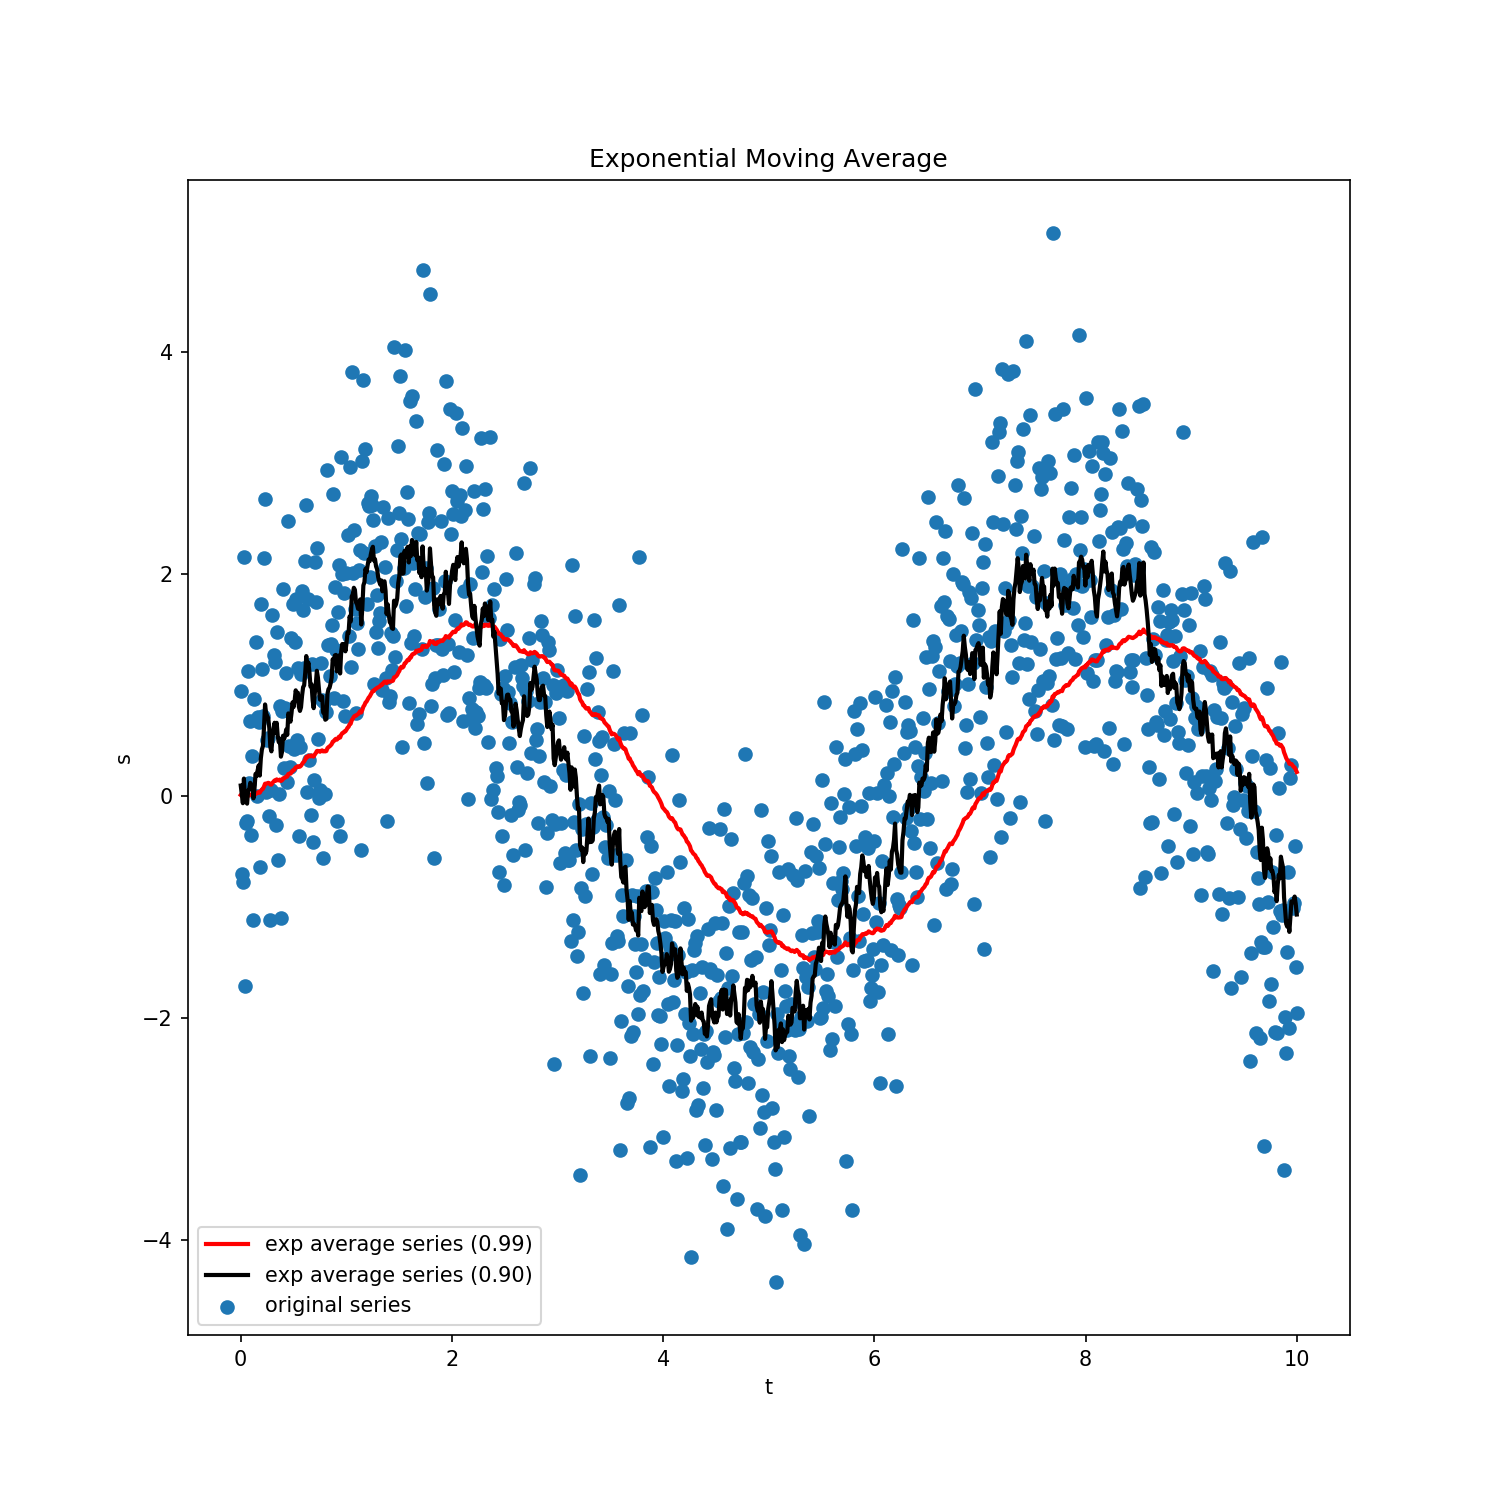
\includegraphics[scale=0.4]{exp_ma_1}
    \centering
    \caption {Exponentially averaged series for different values of $\beta$. Plot prepared using exp\_ma.py.}
    \label{fig:exp_ma_1} %\ref{fig:exp_ma_1}
\end{figure}

Exponential moving average will help approximate a noisy series by a smoother version. Since mini-batch gradient updates are usually a noisy series (since we are not using the entire data to calculate the gradient), the update equation can benefit by this averaging. This is one reason why gradient descent with momentum works.
\begin{align*}
    h_{t} &= \beta h_{t-1} + (1-\beta) \frac{1}{b}\nabla_{w} \sum_{i=1}^{b} L(w_{t-1}, X_{B,i}, Y_{B,i})\\
    w_{t} &= w_{t-1} - \eta h_{t}\\
\end{align*}
Sometimes, another formulation is also used
\begin{align*}
    h_{t} &= \alpha h_{t-1} + \beta \frac{1}{b}\nabla_{w} \sum_{i=1}^{b} L(w_{t-1}, X_{B,i}, Y_{B,i})\\
    w_{t} &= w_{t-1} - h_{t}
\end{align*}
where $\beta$ is different from the one used in the previous formulation (we have multiplied the learning rate in the update equation itself). Both formulation have the same number of parameters. The first one is more intuitive while the second one is a compact form to work with. The learning rates will be different in the two formulations. $\alpha$ is usually $0.9$. Figure \ref{fig:momentum_2} shows a visual representation of this process.\newline

\begin{figure}[h]
    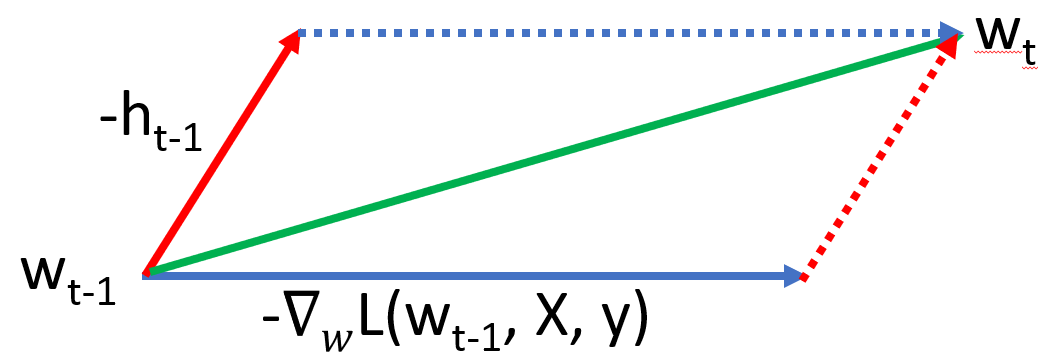
\includegraphics[scale=0.4]{momentum_2}
    \centering
    \caption {Vector representation of Gradient Descent with Momentum}
    \label{fig:momentum_2} %\ref{fig:momentum_2}
\end{figure}

In exponential series, it is often the case to have some bias initially (before smoothing starts). To adjust for this, we use the following transformation
\begin{align*}
    v_{t} = \frac{v_{t}}{1 - \beta^{t}}
\end{align*}
which will be effective only for the first few timesteps. In practice, this correction may not be followed since the average series quickly converges. Figure \ref{fig:exp_ma_1} shows how higher values of $\beta$ give a smoother series, but suffer from high bias as well.\newline

Another reason why gradient descent with momentum works is it's ability to manipulate skewed data. Suppose one dimension of data has more variance than the other. We can expect the loss surface for this to be a highly skewed ellipse. Normal gradient descent will suffer since the gradients in one dimension have high values than the other causing huge oscillations. Momentum helps maintain a single direction of movement (due to averaging) and helps control these oscillations.


%%%%%%%%%%%%%%%%%%%%%%%%%%%%%%
\subsection{Nesterov Momentum (NAG)}
This builds on the concept of momentum and is also known as Nesterov accelerated gradient (NAG). Instead of calculating the gradient using the current value of weights, we calculate is using the future value
\begin{align*}
    h_{t} &= \alpha h_{t-1} + \beta \frac{1}{b}\nabla_{w} \sum_{i=1}^{b} L(w_{t-1} - \alpha h_{t-1}, X_{B,i}, Y_{B,i})\\
    w_{t} &= w_{t-1} - h_{t}
\end{align*}
The reasoning is that momentum may not always point in the correct direction and as such, we correct the direction of the gradient so that the final value of $w$ after update is close to expected. Figure \ref{fig:momentum_3} shows this visually.
\begin{figure}[h]
    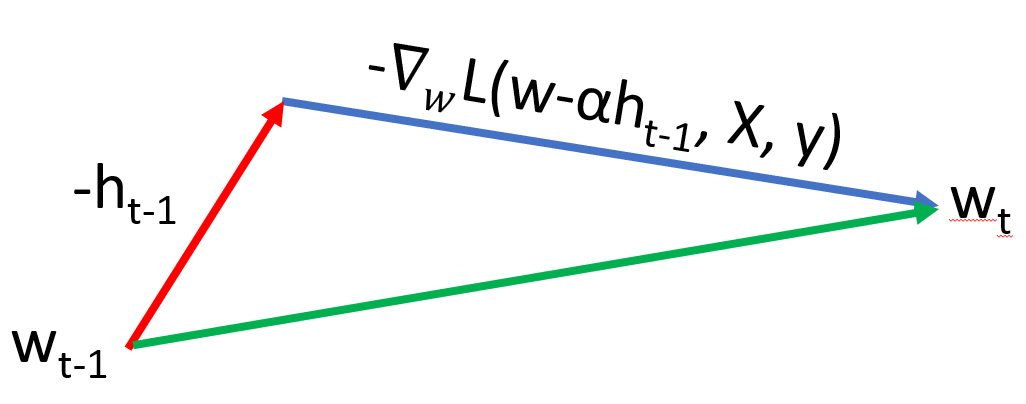
\includegraphics[scale=0.4]{momentum_3}
    \centering
    \caption {Vector representation of Gradient Descent with Nesterov Momentum}
    \label{fig:momentum_3} %\ref{fig:momentum_3}
\end{figure}


%%%%%%%%%%%%%%%%%%%%%%%%%%%%%%
\subsection{AdaGrad}
AdaGrad uses and \emph{adaptive} learning rate to stabilize training. It uses a slightly different value of learning rate for each parameter. Till now, for the entire weight vector $w$, we have used the same learning rate
\begin{align*}
    g_{t,j} &= \nabla_{w_{t-1, j}}L(w_{t-1}, X, y)\\
    G_{t,j} &= G_{t-1,j} + g_{t,j}^{2}\\
    w_{t,j} &= w_{t-1,j} - \frac{\eta}{\sqrt{G_{t,j} + \epsilon}} g_{t,j} 
\end{align*}
where $\eta$ is usually kept fixed at $0.01$, and $G$ keeps increasing with time. Hence, we have an in-built early stopping mechanism where after long time, weight update will stop. The different effective learning rate per parameter, gives us finer control on how weights update.\newline

$\epsilon$ is a small value ($10^{-8}$) kept to prevent denominator from becoming $0$. Due to the accumulation of gradients, the algorithm is not able to learn at large time steps. This can be bad in scenarios like reinforcement learning, where the data might change with timesteps as the agent explores the environment.


%%%%%%%%%%%%%%%%%%%%%%%%%%%%%%
\subsection{RMSProp}
RMSProp is a variation of AdaGrad where the calculation of square of gradient is itself converted to a exponential moving average
\begin{align*}
    g_{t,j} &= \nabla_{w_{t-1, j}}L(w_{t-1}, X, y)\\
    G_{t,j} &= \beta G_{t-1,j} + (1-\beta)g_{t,j}^{2}\\
    w_{t,j} &= w_{t-1,j} - \frac{\eta}{\sqrt{G_{t,j} + \epsilon}} g_{t,j} 
\end{align*}
where $\beta$ is about $0.9$ and $\eta$ about $0.001$, and the exponential average is tracked for every variable individually. Thus, the learning rate also adapts to the latest gradient values because the coefficient $\beta$ will force only a few of the latest gradient values to contribute to the weights update. This is in contrast with AdaGrad where the gradient keeps accumulating and becoming larger, causing the learning rate to continuously decrease.


%%%%%%%%%%%%%%%%%%%%%%%%%%%%%%
\subsection{Adam}
Adam builds on top of RMSProp to bring exponential moving average to the gradient calculation as well. We also have bias correction discussed in section \ref{sec:gradient_descent_momentum}.
\begin{align*}
    g_{t,j} &= \nabla_{w_{t-1, j}}L(w_{t-1}, X, y)\\
    m_{t,j} &= \frac{\beta_{1} m_{t-1,j} + (1-\beta_{1}) g_{t,j}}{1 - \beta_{1}^{t}}\\
    v_{t,j} &= \frac{\beta_{2} v_{t-1,j} + (1-\beta_{2})g_{t,j}^{2}}{1 - \beta_{2}^{t}}\\
    w_{t,j} &= w_{t-1,j} - \frac{\eta}{\sqrt{v_{t,j}} + \epsilon} m_{t,j} 
\end{align*}
We have introduced exponential moving average for both the gradient and it's square, bias correction in both the terms, and also adaptive learning rate. Good initial values are $0.9$ for $\beta_{1}$, $0.999$ for $\beta_{2}$, $10^{-8}$ for epsilon, and $0.1$ for $\alpha$. However, it should be noted that $\alpha$ needs to be tuned differently as per the use case.
\end{document}